\chapter{Hasil dan Pembahasan}

\section{Hasil Pra-Pemrosesan Data}
Bagian ini memaparkan hasil dari setiap tahap pembersihan dan normalisasi data yang telah dilakukan, beserta dampaknya terhadap jumlah dan kualitas data yang digunakan dalam pembangunan graf.

\subsection{Reduksi Jumlah Data}
Proses pra-pemrosesan menyebabkan berkurangnya jumlah baris data secara bertahap akibat penghapusan baris yang tidak valid. Perubahan jumlah data pada tiap tahap ditampilkan pada Tabel~\ref{tab:reduksi-data}.

\begin{table}[H]
\centering
\caption{Reduksi jumlah data pada tiap tahap pra-pemrosesan}
\label{tab:reduksi-data}
\renewcommand{\arraystretch}{1.3}
\begin{tabular}{|c|p{6.5cm}|c|c|}
\hline
\multicolumn{1}{|c|}{\textbf{Tahap}} & \multicolumn{1}{c|}{\textbf{Proses}} & \multicolumn{1}{c|}{\textbf{Jumlah Data}} & \multicolumn{1}{c|}{\textbf{Berkurang}} \\
\hline
1 & Data mentah awal & 650.986 & -- \\
\hline
2 & Penghapusan baris tanpa sanad (No SANAD) & 491.428 & 159.558 \\
\hline
3 & Penghapusan baris dengan elemen \textit{Abu} tunggal & 488.195 & 3.233 \\
\hline
4 & Penghapusan baris diawali kata kekerabatan & 487.451 & 744 \\
\hline
\multicolumn{2}{|c|}{\textbf{Data akhir}} & \textbf{487.451} & \textbf{163.535} \\
\hline
\end{tabular}
\end{table}

Secara keseluruhan, sebanyak 163.535 baris dihapus dari data awal, sehingga tersisa 487.451 baris sanad bersih yang siap digunakan. Penghapusan 159.558 baris tanpa sanad merupakan porsi terbesar dari total reduksi, dan hal ini diperlukan karena baris-baris tersebut tidak memuat informasi relasi periwayatan apa pun sehingga tidak dapat dimodelkan sebagai sisi dalam graf. Apabila dibiarkan, baris ini hanya akan menjadi data kosong yang membebani komputasi tanpa memberikan kontribusi pada jaringan. Adapun penghapusan baris dengan elemen \textit{Abu} tunggal (3.233 baris) dan baris yang diawali kata kekerabatan (744 baris) bertujuan mencegah terbentuknya node ambigu, yaitu elemen seperti \textit{Abu} atau \textit{Abihi} yang berdiri sendiri tanpa nama jelas dan berpotensi menyatukan perawi-perawi berbeda secara keliru ke dalam satu node, sehingga merusak akurasi struktur jaringan dan perhitungan sentralitas.

\subsection{Transformasi Nama Perawi}
\label{subsec:transformasi-nama}
Selain pengurangan jumlah baris, dilakukan pula serangkaian transformasi pada penulisan nama perawi. Contoh hasil sebelum dan sesudah tiap transformasi ditampilkan pada Tabel~\ref{tab:transformasi-nama}. Contoh disajikan dalam bentuk transliterasi Latin; untuk transformasi pada tingkat huruf, jenis huruf yang dinormalisasi dituliskan dalam tanda kurung.

\begin{table}[H]
\centering
\caption{Contoh hasil transformasi nama perawi}
\label{tab:transformasi-nama}
\renewcommand{\arraystretch}{1.3}
\begin{tabular}{|c|p{3.3cm}|p{4.3cm}|p{5cm}|}
\hline
\multicolumn{1}{|c|}{\textbf{No}} & \multicolumn{1}{c|}{\textbf{Proses}} & \multicolumn{1}{c|}{\textbf{Sebelum}} & \multicolumn{1}{c|}{\textbf{Sesudah}} \\
\hline
1 & Penghapusan harakat & \textit{J\=abir bin Zayd} (berharakat) & \textit{Jabir bin Zaid} \\
\hline
2 & Normalisasi alif & \textit{Anas} (alif berhamzah) & \textit{Anas} (alif biasa) \\
\hline
3 & Normalisasi ya & \textit{Musa} (alif maqsura) & \textit{Musa} (ya standar) \\
\hline
4 & Normalisasi ta marbuta & \textit{Aisyah} (ta marbuta) & \textit{Aisyah} (ha) \\
\hline
5 & Resolusi kata kekerabatan & [\textit{Muhammad}, \textit{Abihi}, \textit{Jaddihi}] & [\textit{Muhammad}, \textit{Abu Muhammad}, \textit{Jadd Muhammad}] \\
\hline
\end{tabular}
\end{table}

Setelah seluruh proses normalisasi selesai, diperoleh sebanyak 177.289 nama perawi unik dari keseluruhan rantai sanad. Proses normalisasi ini sangat menentukan keakuratan jumlah node, sebab tanpa normalisasi satu perawi yang sama dapat tersebar menjadi beberapa node berbeda hanya karena variasi penulisan. Sebagai contoh, nama \textit{Aisyah} yang ditulis dengan ta marbuta dan yang ditulis dengan ha akan dihitung sebagai dua perawi terpisah apabila tidak diseragamkan. Dengan menyeragamkan variasi tersebut, setiap node dipastikan merepresentasikan satu perawi unik. Hal ini berdampak langsung pada validitas analisis sentralitas, karena nilai sentralitas seorang perawi hanya akan akurat apabila seluruh relasinya terkonsolidasi dalam satu node, bukan terpecah ke beberapa node duplikat.


\section{Hasil Pembangunan Knowledge Graph Jaringan Sanad}
Bagian ini memaparkan karakteristik graf jaringan sanad yang dihasilkan dari proses pemodelan, meliputi statistik ukuran graf serta cuplikan struktur relasi yang terbentuk.

\subsection{Statistik Graf Jaringan Sanad}
Graf jaringan sanad dibangun sebagai graf berarah (\textit{directed graph}) menggunakan NetworkX. Statistik ukuran graf yang terbentuk ditampilkan pada Tabel~\ref{tab:statistik-graf}.

\begin{table}[H]
\centering
\caption{Statistik graf jaringan sanad}
\label{tab:statistik-graf}
\renewcommand{\arraystretch}{1.3}
\begin{tabular}{|p{7cm}|c|}
\hline
\multicolumn{1}{|c|}{\textbf{Parameter}} & \multicolumn{1}{c|}{\textbf{Nilai}} \\
\hline
Jumlah simpul (\textit{node} / perawi) & 177.047 \\
\hline
Jumlah sisi (\textit{edge} / relasi) & 776.798 \\
\hline
\end{tabular}
\end{table}

Graf jaringan sanad yang terbentuk terdiri dari 177.047 simpul yang merepresentasikan perawi dan 776.798 sisi yang merepresentasikan relasi periwayatan guru--murid. Jumlah simpul dan sisi ini menunjukkan bahwa jaringan sanad yang berhasil dimodelkan berskala besar dan mencakup ratusan ribu jalur periwayatan. Graf inilah yang menjadi dasar bagi perhitungan metrik sentralitas pada tahap analisis berikutnya.

Jumlah simpul tersebut sedikit lebih kecil dibandingkan 177.289 nama perawi unik yang teridentifikasi pada tahap normalisasi nama perawi (Subbab~\ref{subsec:transformasi-nama}). Selisih sebanyak 242 perawi muncul karena perawi-perawi tersebut tidak membentuk relasi apa pun dalam graf, sehingga tidak tercatat sebagai simpul. Kondisi ini terjadi antara lain pada rantai sanad yang hanya memuat satu nama perawi sehingga tidak dapat membentuk pasangan guru--murid, serta pada perawi yang gugur saat pembersihan tahap penyusunan sisi, seperti penghapusan \textit{self-loop} (relasi dengan guru dan murid yang sama) dan penghapusan nama kosong. Dengan demikian, 177.289 menunjukkan jumlah perawi yang teridentifikasi, sedangkan 177.047 menunjukkan jumlah perawi yang benar-benar terlibat dalam minimal satu relasi periwayatan.

\subsection{Hubungan Guru - Murid}
Setiap relasi dalam graf direpresentasikan sebagai tripel (Murid, meriwayatkan-dari, Guru) yang dilengkapi atribut bobot, yaitu \textit{Weight} (frekuensi relasi) dan \textit{Inverse Weight} (kebalikan bobot untuk perhitungan jarak). Relasi guru--murid dengan bobot tertinggi ditampilkan pada Tabel~\ref{tab:relasi-terkuat}.

\begin{table}[H]
\centering
\caption{10 relasi periwayatan dengan bobot tertinggi}
\label{tab:relasi-terkuat}
\renewcommand{\arraystretch}{1.3}
\begin{tabular}{|l|l|c|c|}
\hline
\multicolumn{1}{|c|}{\textbf{Guru}} & \multicolumn{1}{c|}{\textbf{Murid}} & \multicolumn{1}{c|}{\textbf{\textit{Weight}}} & \multicolumn{1}{c|}{\textbf{\textit{Inverse Weight}}} \\
\hline
Ibnu Umar & Nafi' & 11.346 & 0,000088 \\
\hline
Ma'mar & Abdurrazzaq & 6.402 & 0,000156 \\
\hline
Abu Hisyam bin Urwah & Hisyam bin Urwah & 6.390 & 0,000156 \\
\hline
Ibnu Abbas & Ikrimah & 5.456 & 0,000183 \\
\hline
Ibnu Abbas & Sa'id bin Jubair & 4.663 & 0,000214 \\
\hline
Abu Hurairah & Abu Salamah & 4.502 & 0,000222 \\
\hline
Az-Zuhri & Ma'mar & 4.381 & 0,000228 \\
\hline
Abu Hurairah & Abu Shalih & 3.972 & 0,000252 \\
\hline
Aisyah & Urwah & 3.953 & 0,000253 \\
\hline
Aisyah & Abu Hisyam bin Urwah & 3.950 & 0,000253 \\
\hline
\end{tabular}
\end{table}

Tabel~\ref{tab:relasi-terkuat} menunjukkan bahwa relasi terkuat dalam jaringan adalah hubungan antara Ibnu Umar dan Nafi' dengan bobot 11.346, yang berarti Nafi' tercatat meriwayatkan hadis dari Ibnu Umar sebanyak 11.346 kali dalam korpus. Terlihat pula bahwa nilai \textit{Inverse Weight} berbanding terbalik dengan \textit{Weight}, yaitu semakin tinggi frekuensi relasi, semakin kecil nilai \textit{Inverse Weight}-nya. Nilai inilah yang digunakan sebagai representasi jarak dalam perhitungan sentralitas berbasis jalur (\textit{closeness} dan \textit{betweenness}), sehingga pasangan perawi dengan relasi terkuat dianggap memiliki jarak terdekat dalam jaringan. Bobot yang tinggi pada relasi-relasi ini mencerminkan adanya jalur periwayatan utama (\textit{backbone}) yang sangat dominan, yaitu pasangan guru--murid yang konsisten muncul di banyak rantai sanad.

\section{Hasil Analisis Jaringan Sanad (Sentralitas)}
Analisis sentralitas dilakukan untuk mengidentifikasi perawi-perawi yang memiliki peran penting dalam jaringan sanad. Sebelum hasil masing-masing metrik dijelaskan, terdapat cakupan data yang digunakan dalam perhitungan, mengingat tidak seluruh metrik dihitung pada skala data yang sama.

\begin{sloppypar}
Metrik \textit{in-degree centrality}, \textit{out-degree centrality}, dan \textit{eigenvector centrality} dihitung pada graf penuh yang terdiri dari 177.047 simpul dan 776.798 sisi, karena ketiga metrik ini relatif ringan secara komputasi. Sebaliknya, metrik \textit{closeness} dan \textit{betweenness centrality} memerlukan penelusuran jalur terpendek antar seluruh pasangan simpul (\textit{all-pairs shortest path}) yang berbiaya komputasi sangat tinggi sehingga tidak memungkinkan dijalankan pada graf penuh. Oleh karena itu, kedua metrik tersebut dihitung pada subset data, yaitu 50.000 relasi dengan bobot tertinggi yang membentuk subgraf berisi 14.695 simpul. Rincian cakupan data tiap metrik ditampilkan pada Tabel~\ref{tab:cakupan-metrik}.
\end{sloppypar}

\begin{table}[H]
\centering
\caption{Cakupan data perhitungan tiap metrik sentralitas}
\label{tab:cakupan-metrik}
\renewcommand{\arraystretch}{1.3}
\begin{tabular}{|l|l|c|c|}
\hline
\multicolumn{1}{|c|}{\textbf{Metrik}} & \multicolumn{1}{c|}{\textbf{Cakupan Data}} & \multicolumn{1}{c|}{\textbf{Jumlah Simpul}} & \multicolumn{1}{c|}{\textbf{Jumlah Sisi}} \\
\hline
\textit{In-Degree Centrality} & Graf penuh & 177.047 & 776.798 \\
\hline
\textit{Out-Degree Centrality} & Graf penuh & 177.047 & 776.798 \\
\hline
\textit{Eigenvector Centrality} & Graf penuh & 177.047 & 776.798 \\
\hline
\textit{Closeness Centrality} & Subset (bobot tertinggi) & 14.695 & 50.000 \\
\hline
\textit{Betweenness Centrality} & Subset (bobot tertinggi) & 14.695 & 50.000 \\
\hline
\end{tabular}
\end{table}

Penggunaan subset untuk \textit{closeness} dan \textit{betweenness} tetap representatif karena 50.000 relasi dengan bobot tertinggi mewakili jalur-jalur periwayatan utama yang paling sering muncul dalam korpus, sehingga perawi-perawi sentral tetap dapat teridentifikasi dengan baik.

\begin{enumerate}
	\item \textbf{In Degree Centrality}

	\textit{In-degree centrality} mengukur jumlah murid yang meriwayatkan dari seorang perawi, sehingga menunjukkan perannya sebagai sumber riwayat (guru). Sepuluh perawi dengan nilai tertinggi ditampilkan pada Gambar~\ref{fig:top-indegree}.

	\begin{figure}[H]
	\centering
	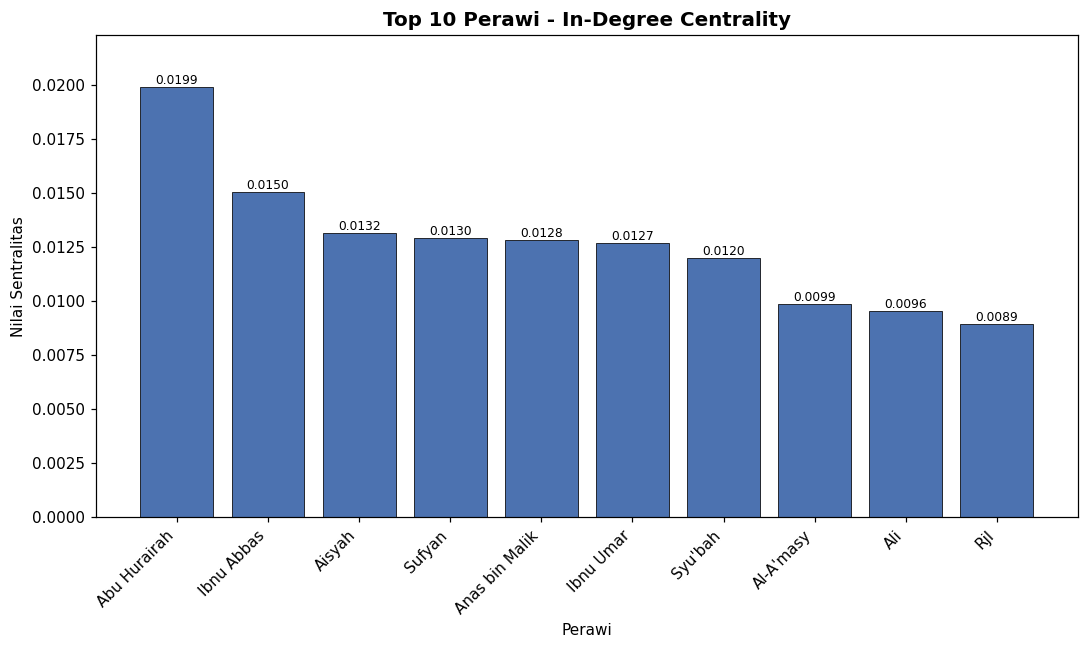
\includegraphics[width=0.9\textwidth]{contents/chapter-4/In-degree.png}
	\caption{Sepuluh perawi dengan \textit{in-degree centrality} tertinggi}
	\label{fig:top-indegree}
	\end{figure}

	Berdasarkan Gambar~\ref{fig:top-indegree}, Abu Hurairah menempati posisi tertinggi dengan nilai \textit{in-degree centrality} sebesar 0,0199, diikuti oleh Ibnu Abbas (0,0150) dan Aisyah (0,0132). Nilai \textit{in-degree} yang tinggi menunjukkan bahwa perawi tersebut memiliki jumlah murid terbanyak, yaitu paling banyak menjadi sumber periwayatan bagi perawi lain dalam jaringan. Nilai sentralitas menurun secara bertahap dari peringkat pertama hingga peringkat kesepuluh yang bernilai 0,0089, dengan selisih yang cukup mencolok antara Abu Hurairah dan perawi-perawi di bawahnya. Pola ini menunjukkan bahwa peran sebagai sumber riwayat dominan terkonsentrasi pada sejumlah kecil perawi yang berada di puncak jaringan.

	\item \textbf{Out Degree Centrality}

	\textit{Out-degree centrality} mengukur jumlah guru yang menjadi sumber riwayat bagi seorang perawi, sehingga menunjukkan perannya sebagai penerima riwayat (murid) yang aktif. Sepuluh perawi dengan nilai tertinggi ditampilkan pada Gambar~\ref{fig:top-outdegree}.

	\begin{figure}[H]
	\centering
	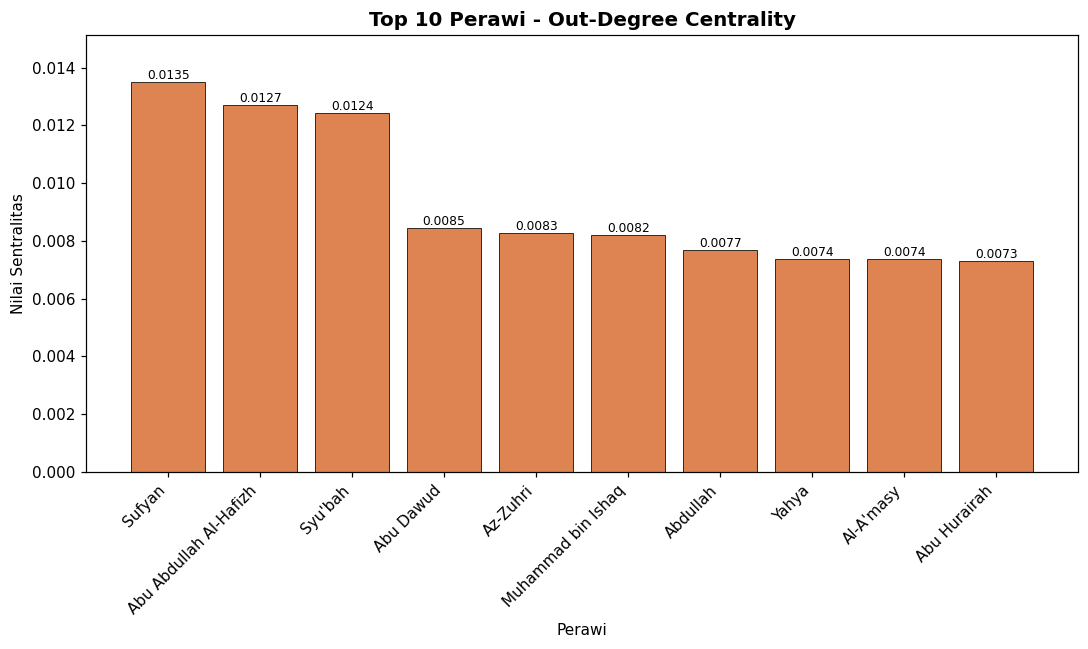
\includegraphics[width=0.9\textwidth]{contents/chapter-4/Out-degree.png}
	\caption{Sepuluh perawi dengan \textit{out-degree centrality} tertinggi}
	\label{fig:top-outdegree}
	\end{figure}

	Berdasarkan Gambar~\ref{fig:top-outdegree}, Sufyan menempati posisi tertinggi dengan nilai \textit{out-degree centrality} sebesar 0,0135, diikuti oleh Abu Abdullah Al-Hafizh (0,0127) dan Syu'bah (0,0124). Nilai \textit{out-degree} yang tinggi menunjukkan bahwa perawi tersebut meriwayatkan dari banyak guru yang berbeda, sehingga berperan sebagai penerima riwayat yang aktif dalam jaringan. Nilai sentralitas menurun dari peringkat pertama hingga peringkat kesepuluh yang bernilai 0,0073. Susunan perawi pada metrik ini berbeda dari \textit{in-degree centrality}, yang menandakan bahwa perawi yang dominan sebagai sumber riwayat tidak selalu sama dengan perawi yang dominan sebagai penerima riwayat.

	\item \textbf{Eigenvector Centrality}

	\textit{Eigenvector centrality} mengukur pengaruh seorang perawi berdasarkan kualitas koneksinya, yaitu keterhubungan dengan perawi-perawi lain yang juga berpengaruh. Sepuluh perawi dengan nilai tertinggi ditampilkan pada Gambar~\ref{fig:top-eigenvector}.

	\begin{figure}[H]
	\centering
	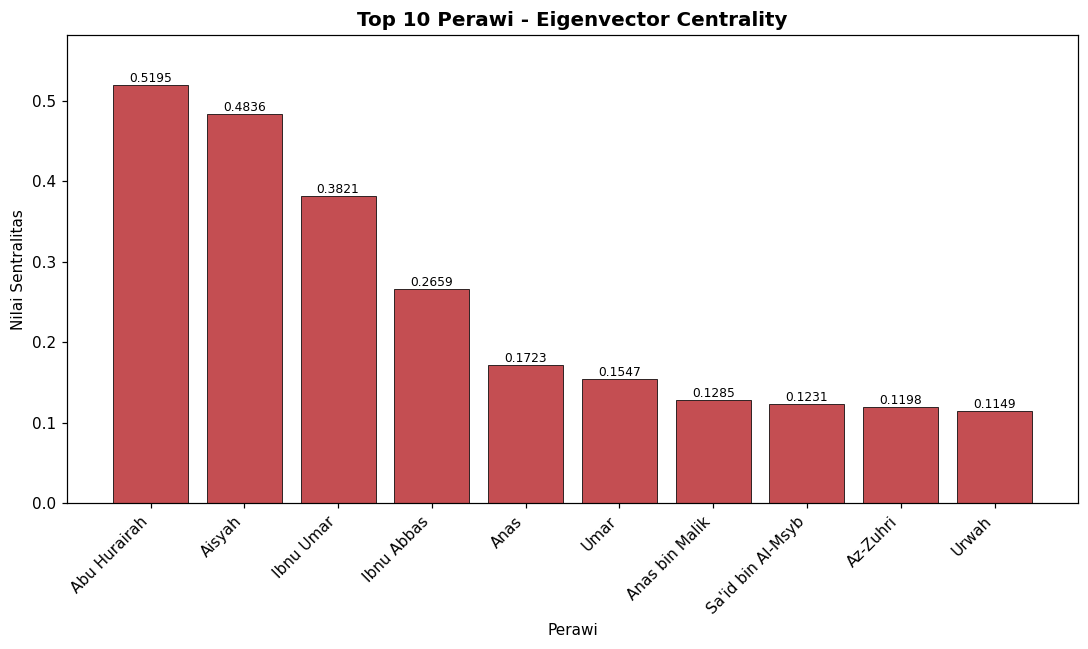
\includegraphics[width=0.9\textwidth]{contents/chapter-4/Eigenvector.png}
	\caption{Sepuluh perawi dengan \textit{eigenvector centrality} tertinggi}
	\label{fig:top-eigenvector}
	\end{figure}

	Berdasarkan Gambar~\ref{fig:top-eigenvector}, Abu Hurairah menempati posisi tertinggi dengan nilai \textit{eigenvector centrality} sebesar 0,5195, diikuti oleh Aisyah (0,4836) dan Ibnu Umar (0,3821). Nilai yang tinggi menunjukkan bahwa perawi tersebut terhubung dengan perawi-perawi lain yang juga memiliki pengaruh tinggi dalam jaringan. Terlihat adanya penurunan nilai yang tajam setelah empat peringkat teratas, yaitu dari 0,2659 (Ibnu Abbas) menjadi 0,1723 (Anas) dan seterusnya hingga 0,1149 pada peringkat kesepuluh. Pola ini menunjukkan bahwa pengaruh dalam jaringan terkonsentrasi pada sejumlah kecil perawi yang saling terhubung erat di pusat jaringan.

	\item \textbf{Closeness Centrality}

	\textit{Closeness centrality} mengukur kedekatan seorang perawi terhadap seluruh perawi lain berdasarkan rata-rata jarak terpendek. Metrik ini dihitung pada subgraf berisi 14.695 simpul dengan bobot relasi tertinggi. Sepuluh perawi dengan nilai tertinggi ditampilkan pada Gambar~\ref{fig:top-closeness}.

	\begin{figure}[H]
	\centering
	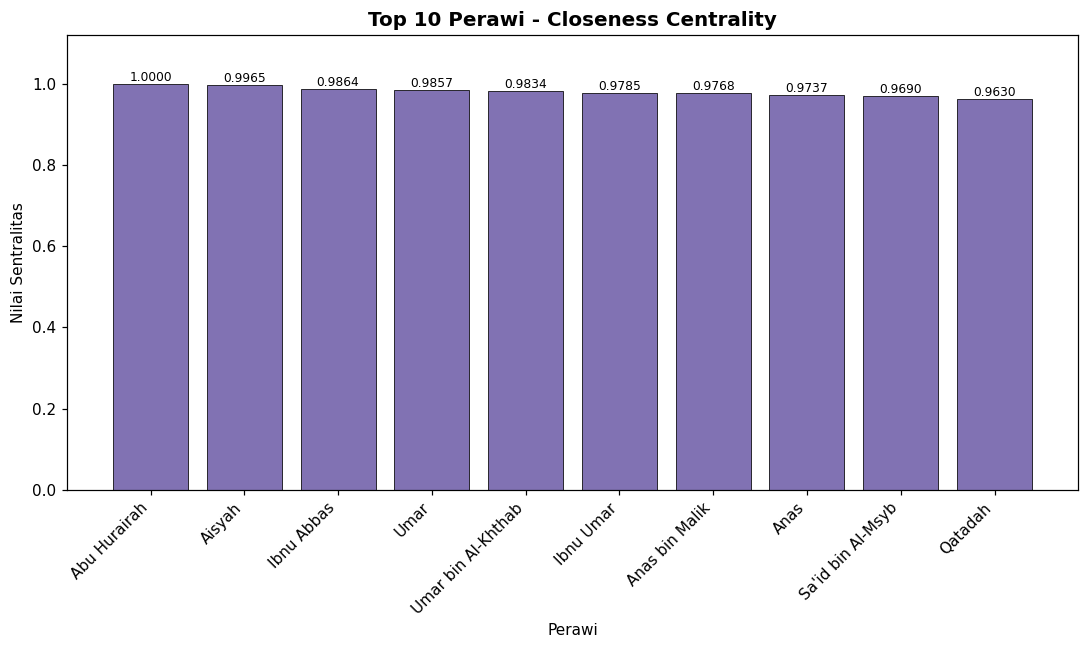
\includegraphics[width=0.9\textwidth]{contents/chapter-4/Closeness.png}
	\caption{Sepuluh perawi dengan \textit{closeness centrality} tertinggi}
	\label{fig:top-closeness}
	\end{figure}

	Berdasarkan Gambar~\ref{fig:top-closeness}, Abu Hurairah menempati posisi tertinggi dengan nilai \textit{closeness centrality} sebesar 1,0000, diikuti oleh Aisyah (0,9965) dan Ibnu Abbas (0,9864). Nilai kesepuluh perawi teratas sangat tinggi dan saling berdekatan, yaitu berada pada rentang 0,9630 hingga 1,0000. Kedekatan nilai ini menunjukkan bahwa pada subgraf relasi terkuat, perawi-perawi teratas dapat menjangkau perawi lain melalui jalur periwayatan yang sangat pendek, sehingga menempati posisi yang sentral dalam penyebaran riwayat.

	\item \textbf{Betweenness Centrality}

	\textit{Betweenness centrality} mengukur seberapa sering seorang perawi berada pada jalur terpendek antara pasangan perawi lain, sehingga menunjukkan perannya sebagai penghubung dalam jaringan. Metrik ini juga dihitung pada subgraf berisi 14.695 simpul dengan bobot relasi tertinggi. Sepuluh perawi dengan nilai tertinggi ditampilkan pada Gambar~\ref{fig:top-betweenness}.

	\begin{figure}[H]
	\centering
	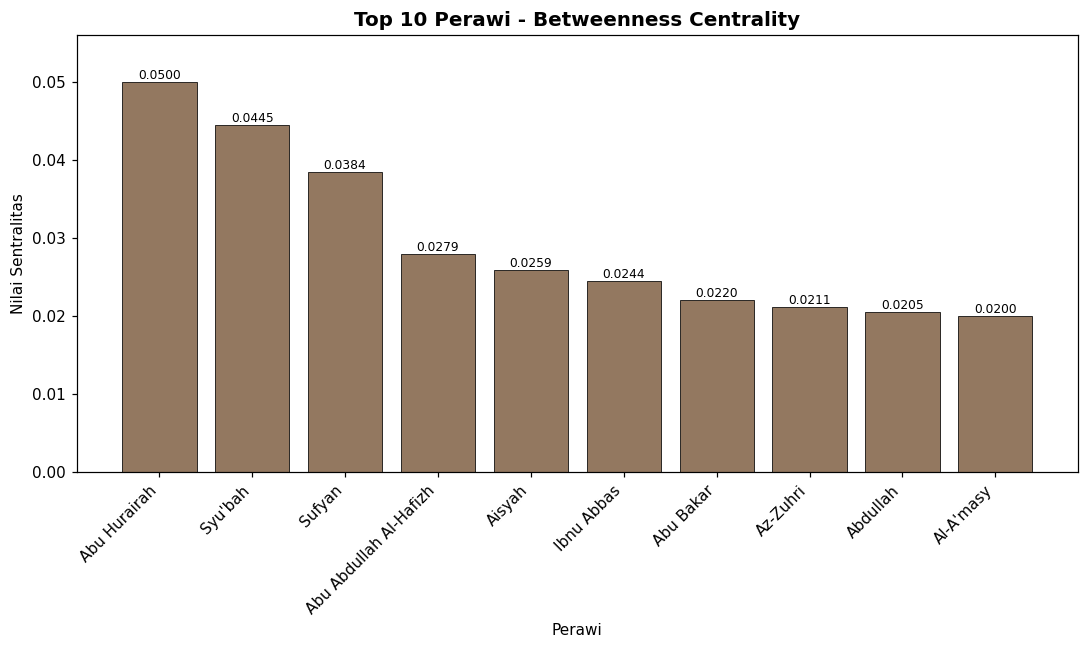
\includegraphics[width=0.9\textwidth]{contents/chapter-4/Betweenn.png}
	\caption{Sepuluh perawi dengan \textit{betweenness centrality} tertinggi}
	\label{fig:top-betweenness}
	\end{figure}

	Berdasarkan Gambar~\ref{fig:top-betweenness}, Abu Hurairah menempati posisi tertinggi dengan nilai \textit{betweenness centrality} sebesar 0,0500, diikuti oleh Syu'bah (0,0445) dan Sufyan (0,0384). Nilai yang tinggi menunjukkan bahwa perawi tersebut sering menjadi titik perlintasan pada jalur terpendek antar-perawi, sehingga berperan sebagai penghubung dalam jaringan. Nilai sentralitas menurun secara bertahap hingga 0,0200 pada peringkat kesepuluh. Peringkat teratas pada metrik ini memuat perawi yang juga muncul pada metrik lain, seperti Abu Hurairah, Syu'bah, dan Sufyan, yang menandakan peran ganda mereka baik sebagai simpul berpengaruh maupun sebagai penghubung antar-bagian jaringan.
\end{enumerate}

\section{Hasil Penyimpanan Data ke Supabase}
Hasil analisis yang telah diekspor menjadi berkas CSV selanjutnya diunggah ke basis data Supabase. Data disusun ke dalam dua tabel relasional, yaitu tabel Sentralitas yang memuat data perawi beserta nilai metriknya dan tabel Edge yang memuat data relasi periwayatan. Hasil penyimpanan kedua tabel pada \textit{Table Editor} Supabase ditunjukkan pada Gambar~\ref{fig:supabase-sentralitas} dan Gambar~\ref{fig:supabase-edge}.

\begin{figure}[H]
	\centering
	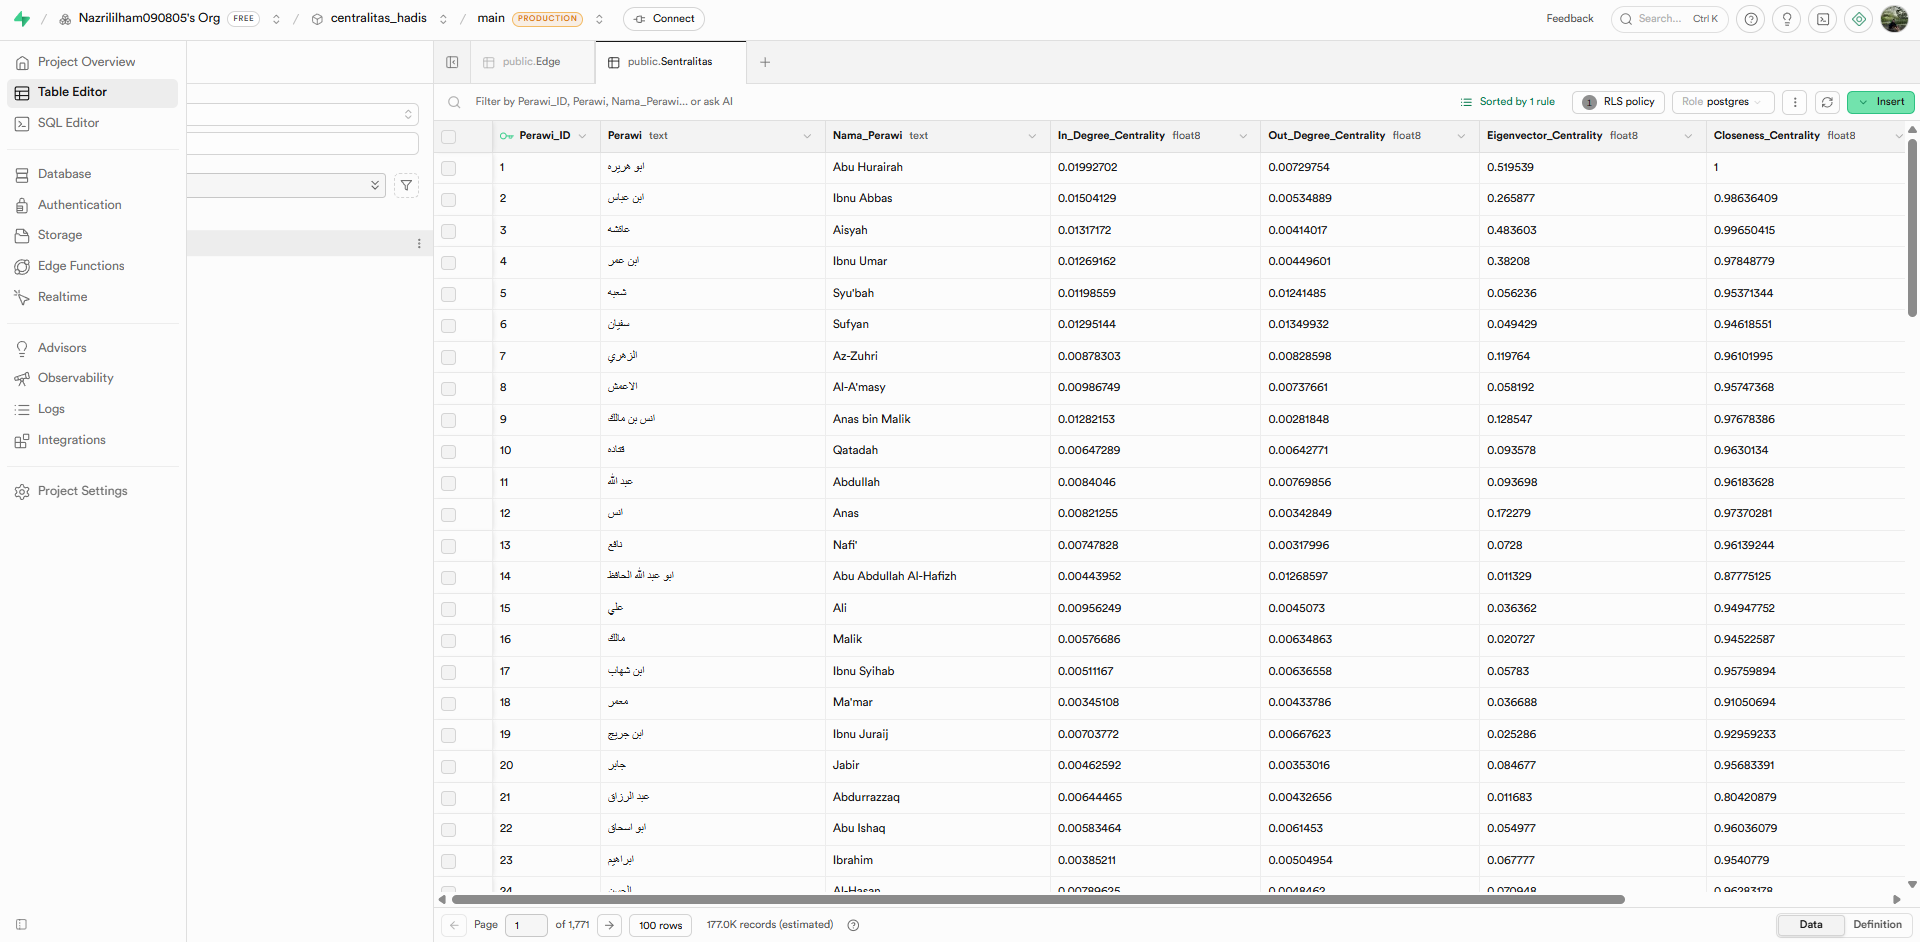
\includegraphics[width=\textwidth]{contents/chapter-4/SentralitasSupabase.png}
	\caption{Tabel Sentralitas pada Supabase}
	\label{fig:supabase-sentralitas}
\end{figure}

\begin{figure}[H]
	\centering
	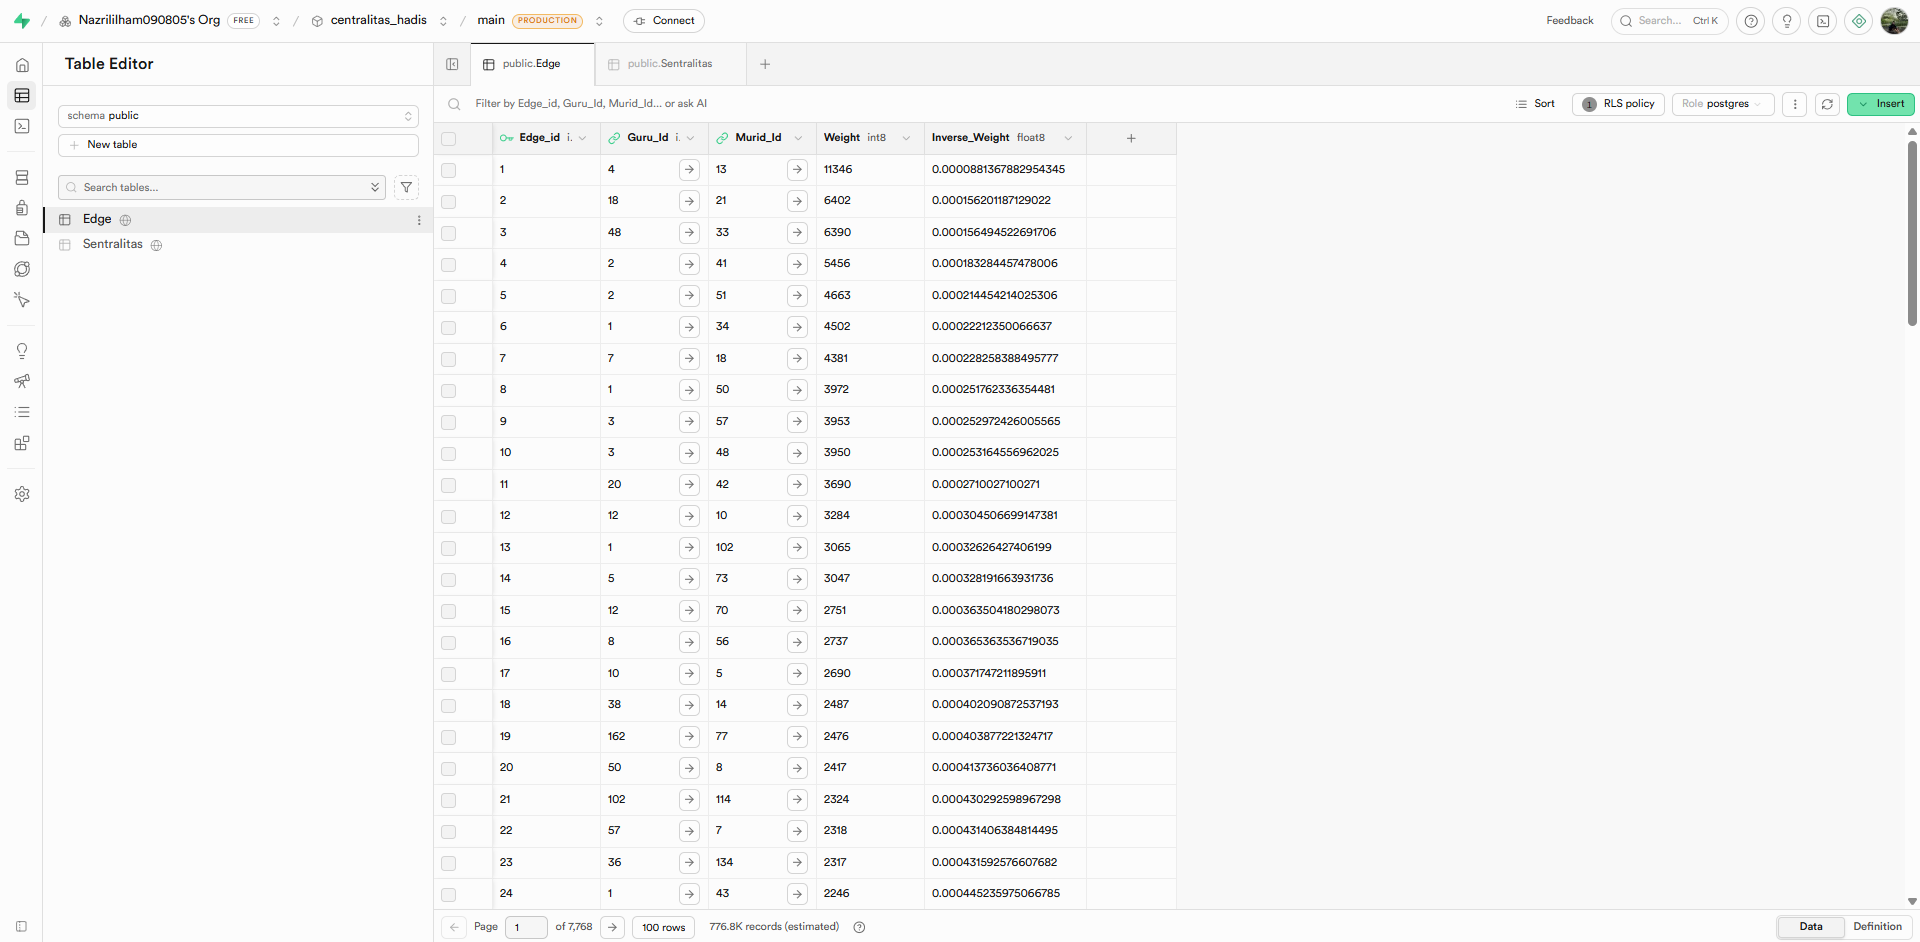
\includegraphics[width=\textwidth]{contents/chapter-4/EdgeSupabase.png}
	\caption{Tabel Edge pada Supabase}
	\label{fig:supabase-edge}
\end{figure}

Gambar~\ref{fig:supabase-sentralitas} memperlihatkan tabel Sentralitas yang memuat data setiap perawi sebagai simpul, dengan kolom Perawi\_ID sebagai kunci primer, Nama\_Perawi (nama dalam aksara Latin), Perawi (nama dalam aksara Arab), serta kelima kolom nilai metrik sentralitas, yaitu In\_Degree\_Centrality, Out\_Degree\_Centrality, Eigenvector\_Centrality, Closeness\_Centrality, dan Betweenness\_Centrality. Sementara itu, Gambar~\ref{fig:supabase-edge} memperlihatkan tabel Edge yang memuat data relasi periwayatan, dengan kolom Edge\_id sebagai kunci primer, Guru\_Id dan Murid\_Id yang merujuk pada Perawi\_ID di tabel Sentralitas, serta Weight sebagai bobot relasi. Keterhubungan melalui Guru\_Id dan Murid\_Id inilah yang menjadikan kedua tabel saling berelasi, sehingga sistem dapat menelusuri jaringan sanad secara utuh.

Proses impor berlangsung dengan benar, ditandai oleh keberhasilan pemetaan setiap kolom (\textit{header}) pada berkas CSV menjadi kolom pada tabel basis data, serta tersimpannya setiap baris CSV sebagai satu \textit{record} tanpa kehilangan data. Penyimpanan hasil analisis ke dalam basis data ini menerapkan pemisahan antara proses komputasi dan proses penyajian. Seluruh perhitungan yang berat dilakukan satu kali secara \textit{offline}, kemudian hasil akhirnya disimpan di Supabase, sehingga \textit{dashboard} cukup mengambil data yang sudah jadi melalui \textit{REST API} tanpa perlu menghitung ulang. Pendekatan ini membuat \textit{dashboard} dapat berjalan ringan dan responsif ketika mengakses data hasil analisis.

\section{Implementasi Sistem Dashboard}
% Pengantar: dashboard hasil implementasi dari rancangan Bab III.

\begin{enumerate}
	\item \textbf{Halaman Graf Relasi Perawi}
	% Screenshot halaman. Jelaskan implementasi visualisasi graf interaktif:
	% algoritma tata letak force-directed dan rendering dengan HTML5 Canvas,
	% interaksi (zoom, drag, klik node -> panel detail), pewarnaan/ukuran node per metrik.

	\item \textbf{Halaman Statistik Perawi}
	% Screenshot. Jelaskan kartu Total Perawi/Relasi dan lima diagram batang Top sentralitas.

	\item \textbf{Halaman Tabel Relasi}
	% Screenshot. Jelaskan penyajian data relasi (guru, murid, weight) + fitur pencarian.

	\item \textbf{Halaman Tabel Sentralitas}
	% Screenshot. Jelaskan penyajian data perawi + kelima metrik + fitur pencarian.
\end{enumerate}

\section{Pengujian Sistem}
% Tabel hasil pengujian black-box: salin skenario dari Tabel pengujian Bab III,
% tambahkan kolom Hasil Aktual dan Status (Valid/Tidak). Bahas tingkat keberhasilan.

\section{Perbandingan Hasil Penelitian dengan Hasil Terdahulu}
% Tabel perbandingan dengan penelitian terdahulu (mis. Mghari et al., CHN Visualizer):
% aspek data, metrik SNA, dan ketersediaan front-end interaktif.
% Bahas kelebihan dan keterbatasan dibanding penelitian/produk lain.
